\documentclass[11pt]{article}
\usepackage{amsmath, amssymb}
\usepackage{geometry}
\geometry{margin=1in}
\usepackage{fancyhdr}
\usepackage{lastpage}
\usepackage{parskip} % Better paragraph spacing
\usepackage{titlesec} % Better section formatting
\usepackage{graphicx}
\usepackage{float}
\usepackage[most]{tcolorbox}
\usepackage{lmodern}
\usepackage{caption}
\usepackage{hyperref}

% Define commands for reusable content
\newcommand{\coursename}{COM-402 Information Security and Privacy}
\newcommand{\lecturenum}{07}
\newcommand{\lecturedate}{\today}
\newcommand{\professor}{Mathias Payer}

\hypersetup{colorlinks=true,linkcolor=blue,urlcolor=blue}

% Configure section spacing
\titlespacing*{\section}{0pt}{2ex plus 1ex minus .2ex}{1.5ex plus .2ex}
% Header / Footer
\pagestyle{fancy}
\fancyhf{}
\fancyhead[L]{\coursename}
\fancyhead[R]{Lecture \lecturenum}
\fancyfoot[L]{EPFL - Computer Science}
\fancyfoot[C]{Author: Jonathan Dutoit}
\fancyfoot[R]{Page \thepage\ of \pageref{LastPage}}

\begin{document}

\begin{center}
  {\large EPFL - Computer Science} \\[0.5em]
  {\Large \textbf{\coursename}} \\[0.5em]
  {\large Lecture \lecturenum\ --- \lecturedate} \\[0.5em]
  {\large Author: Jonathan Dutoit} \\[0.5em]
  {\large Professor: \professor} \\[0.5em]
\end{center}

\vspace{2cm}

\begin{center}
  {\LARGE \textbf{Automated Testing}}
\end{center}

\vspace{1cm}

\section*{Learning goals for today}

\begin{itemize}
	\item Differentiate between testing approaches (manual, semi-automatic, automatic)
	\item Leverage fuzzing as a software testing technique
	\item Understand input generation and mutation to effectively explore targets 
	\item Learn about sanitization methods to detect more bugs
	\item Identify opportunities for improving fuzzers
	\item Explain bug oracles and how they signal faults
\end{itemize}

Third-party library vulnerabilities can propagate to commercial software and be used for exploitation, e.g., in Chrome. A bug in a third-party component corrupts memory in the renderer process. 

\textbf{Why testing?}

Testing is the process of analysing a program to find errors. An error is simply a deviation between observed behavior and specified behavior, i.e., a violation of the underlying specification: 

\begin{itemize}
	\item Functional requirements (features a, b, c)
	\item Operational requirements (performance, usability)
	\item What about security requirements?
\end{itemize}

\textbf{Testing can only show the presence of bugs, never their absence}!

\begin{tcolorbox}[
  colback=gray!15,     % background color
  colframe=black!50,    % border color
  boxrule=1pt,       % border thickness
  arc=3mm,             % rounded corners
  left=4mm, right=4mm, top=2mm, bottom=2mm % padding
]
\textbf{(Edsger W. Dijkstra)}

\vspace{0.3cm}

A successful test find a deviation. Testing is a form of program analysis. Code is analyzed, the testing environment observers the behavior of the code, detecting violations. 

\end{tcolorbox}

\section*{Turtles All the Way Down: Bugs are Everywhere}

Giant code bases
\begin{itemize}
	\item Chromium, Linux Kernel, GNOME, etc...
	\item Millions of LoC result in a huge attack surface
	\item Millions of vulnerable hosts, bug is weaponizable 
\end{itemize}

Dependency inflation
\begin{itemize}
	\item X depends-on {A depends-on {1 depends-on ...}, ...}
	\item Redundant code, even bigger attack surface
	\item Single point-of-failure (e.g., Log4j)
\end{itemize}

System abstraction
\begin{itemize}
	\item Developers unaware of underlying assumptions
	\item ChatGPT-generated code
\end{itemize}

Integration hell
\begin{itemize}
	\item 2 "bug-free" systems can still interact in a faulty manner
\end{itemize}

\section*{Software Testing and Verification}

Manual Testing: done manually by the developer
\begin{itemize}
	\item Code reviews
	\item Unit and regression tests (JUnit, libcheck) are incomplete but sound, only code with tests is tested but any failed tests indicate an actual issue
\end{itemize}

Semi-automated Testing: combines manual efforts with automated tools
\begin{itemize}
	\item Annotation (pre- and post-conditions) and proof engines (F* lang)
	\item Type checking and dependent types (Coq, F*)
	\item Code bug pattern search (CodeQL) 
\end{itemize}

Automated Testing: relies on automated tools without a human-in-the-loop
\begin{itemize}
	\item Static analysis is neither sound (only reports true bugs) nor complete (report all bugs) due to lack of runtime information but remains an indicator of possible bugs. 
	\item Dynamic analysis (\textbf{fuzzing}, symbolic execution) is incomplete but sound due to state explosion but any report issues are true bugs. 
\end{itemize}

\vspace{0.5cm}

\begin{center}
  {\LARGE \textbf{Manual Testing}}
\end{center}
\vspace{0.5cm}

\section*{Code Reviews}
Code review improves software quality through peer review, i.e., reviewers read (parts of) the code and specification to find flaws and to highlight code smells
\begin{itemize}
	\item Flaw: any violation of the specification or bug
	\item Code smells: not per-se an issue but could become one (target to improve)
\end{itemize}

Goals: improve code quality, find flaws, learning/knowledge transfer, foster ideas/alternate solutions, complicate to standards (e.g., standards may require certain code reviews)

Code reviews can never find all flaws, but offer different thoroughness. Different types of code reviews: inspection, walk-through, or audit.

\section*{Types of Code Reviews: Inspection}

During an \textbf{inspection}, a group of reviewers goes through all code line-by-line to find flaws and to document any unexpected behavior. 
\begin{itemize}
	\item Multiple developers thoroughly review code
	\item All interactions with dependencies are inspected
	\item Validates current snapshot of code base
	\item "Stop the world" form of code review, as no concurrent progress possible
	\item Most thorough form of code review (but also most expensive)
	\item Goal: sporadically check and review all code
\end{itemize}

\section*{Types of Code Reviews: Walk-through}

In a \textbf{walk-through}, whenever a new feature is available, check that feature and how it interacts with the rest of the system. 
\begin{itemize}
	\item Code is reviewed incrementally, assumes the rest of the code remains correct
	\item Gradual reviews of code base, focusing on new code
	\item Review changes (i.e., pull requests or commits), before they are integrated
	\item Better suited to modern project development
	\item Pioneered by Google's code review practices
	\item Focus is on improving code quality
	\item Goal: continuously validate code as it is integrated
\end{itemize}

\section*{Types of Code Reviews: Audit}

During an \textbf{audit}, a (often external) group of reviewers spot-checks the code to find flaws, often searching patterns to find flaws/violations
\begin{itemize}
	\item Not all code is checked, but spot checks identify issues
	\item Assign fixed amount of time, assume incompleteness
	\item Audits focus on key issues, not fine details
	\item Goal: get an overview of code quality and identify main flaws
\end{itemize}

\section*{Unit and Regression Tests}

A \textbf{unit test}, executes and tests a fragment of code (e.g., function or file). 

Developers write unit tests alongside the functional code to quickly test it during development. There are \textit{positive} tests to ensure code accept and correctly processes valid input and \textit{negative} tests to ensure code rejects invalid inputs. 

Whenever code is changed, unit tests are run to protect against regression. 

When finding a bug, add a unit test to trigger the bug and test that the bug is correctly fixed to protect against \textbf{regression}.


\vspace{0.5cm}

\begin{center}
  {\LARGE \textbf{Semi-Automated Testing}}
\end{center}
\vspace{0.5cm}

\section*{Static Analysis: Compile Time Warnings}

Goal: highlight issues in code, give feedback to developer

Must be fast (low overhead, simple analysis) and must have low false positives (warning fatigue). 

\verb|clang -Wall -Wextra -Wpedantic|

\begin{itemize}
	\item Wall: enables basic set of warnings, mostly easy to fix
	\item Wextra: extends Wall, being a little more detailed; examples are empty function bodies, unused parameters, or sign mismatches
	\item Wpedantic: warns about anything that goes beyond strict C/C++, highlights areas of bad code style as well
	\item Weverything: turn on every single warning that exists; creates noise
\end{itemize}

\section*{Static Analysis}

A static analysis reasons about the code of executing it. 

The line between static and dynamic analysis is blurry. Generally: a static analysis looks only at the code without keeping track of concrete values during execution. 

Advantage of static analysis: 
\begin{itemize}
	\item Full coverage (no need for complete test cases)
	\item Scales to large code bases (but test cases may miss edge cases)
	\item Abstract interpretation (no need for a runtime environment)
\end{itemize}

Disadvantage (having a lot of false positives): 
\begin{itemize}
	\item Computation depends on data, resulting in undecidability 
	\item Over-approximation due to imprecision and aliasing leading to false positives
\end{itemize}

\section*{Annotations}

Annotations augment source doe but are not part of the functional code itself. Compilers may use annotations to test or check certain properties. For example: 
\begin{itemize}
	\item Types in python
	\item Argument usage in C/C++
	\item Pre/postconditions for verification
\end{itemize}

\section*{CodeQL: Analysis Framework to Find Bugs}

CodeQL is a pattern-based code analysis engine to automate security checks. Target code is parsed and analyzed based on patterns in the query language, starting from sources the patterns search for a path towards a sink. 

Analysis is performed on a database that stores all the \textbf{compilation information}

Quality of the reported bugs depends on the quality of the queries (heuristics)

\section*{SemGrep: Find bugs variants with source-code patterns}

SemGrep is a lightweight static analysis tool for bug discovery. It's similar to CodeQL, finds vulnerable code that match an input pattern. 

It \textbf{does not require compilation}. On the other hand, it cannot reason about \textbf{variable types}.

\section*{The 8 "Laws" of Static Analysis}

\begin{itemize}
	\item Can't check code you don't see: must fit into build system
	\item Can't check code you can't parse: must parse "real" code
	\item Not everything is implemented in C: must handle other languages
	\item Not a bug: developers will not fix any report
	\item Not all bugs matter: developers must prioritize
	\item False positives matter: reduce developer burden
	\item False negatives matters: reduce developer burden
	\item Annotations are extremely costly: reduce developer burden
\end{itemize}

\vspace{0.5cm}

\begin{center}
  {\LARGE \textbf{Automated Testing}}
\end{center}
\vspace{0.5cm}

\section*{Formal Verification: Model Checking / Symbolic Execution}

\begin{tcolorbox}[
  colback=yellow!15,     % background color
  colframe=black!50,    % border color
  boxrule=1pt,       % border thickness
  arc=3mm,             % rounded corners
  left=4mm, right=4mm, top=2mm, bottom=2mm % padding
]
Instead of running the program, translate it into a formula, and ask constraint solver about violation on all feasible/possible paths
\end{tcolorbox}

\section*{Formal Verification}

Formal verification is the act of \textbf{\textit{proving}} or disproving the \textbf{\textit{correctness of a system}} with respect to a certain formal specification or property

\begin{itemize}
	\item Model checking: translate code into state machine, model checker analyzes state machine
	\item Symbolic execution: engine analyzes program by exploring paths
\end{itemize}

\section*{(Bounded) Model Checking}

The analyst translates the code and specification into a finite state machine. The model checker then verifies that no illegal states are reachable. 

While this allows end-to-end verification, it is highly labor intensive. 

\textcolor{red}{\textbf{Bounded model}} checking slices the program end checks the slices instead to scale a bit further (1000s LoC instead of 100s LoC)

It's useful for small software: pacemeaker, etc...
\textbf{It doesn't scale to large software!}

\section*{Symbolic Execution}

Values treated as symbols without concrete values. 

Define set of conditions at code locations
\begin{itemize}
	\item Symbolic Execution determines triggering input
\end{itemize}

Testing: finding bugs in applications
\begin{itemize}
	\item Infer pre/post conditions and add assertions
	\item Use symbolic execution to negate conditions
\end{itemize}

Generating PoC input through SAT/SMT solving
% Quick centered image
\begin{figure}[H]
    \centering
    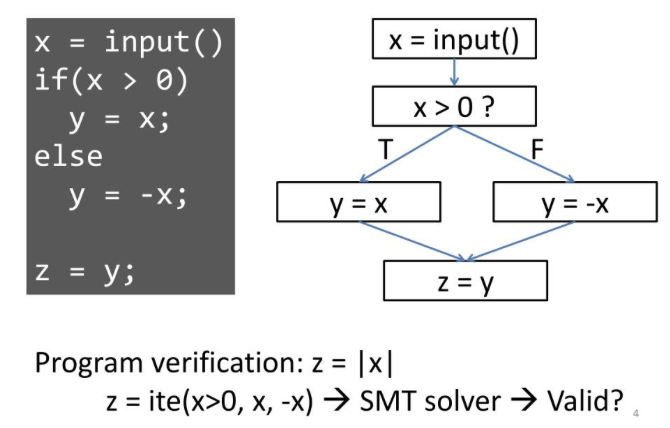
\includegraphics[width=0.8\textwidth]{symbolic-exec}
    \label{fig:LABEL}
\end{figure}
\section*{Symbolic Execution: Challenges}

Bug conditions must be clearly defined. 

\textbf{\textit{State explosion}}: either the length of the constraints or the amount of state doubles at each loop iteration/conditional
\begin{itemize}
	\item Searching valid paths (depth/breadth first) is crucial
	\item Path optimization key research are
	\item State pruning another key are
\end{itemize}

Complexity limits scalability. 

\begin{tcolorbox}[
  colback=yellow!15,     % background color
  colframe=black!50,    % border color
  boxrule=1pt,       % border thickness
  arc=3mm,             % rounded corners
  left=4mm, right=4mm, top=2mm, bottom=2mm % padding
]
Symbolic execution is complete in theory (when all paths are checked) but incomplete in practice (due to state explosion)

\end{tcolorbox}

% Quick centered image
\begin{figure}[H]
    \centering
    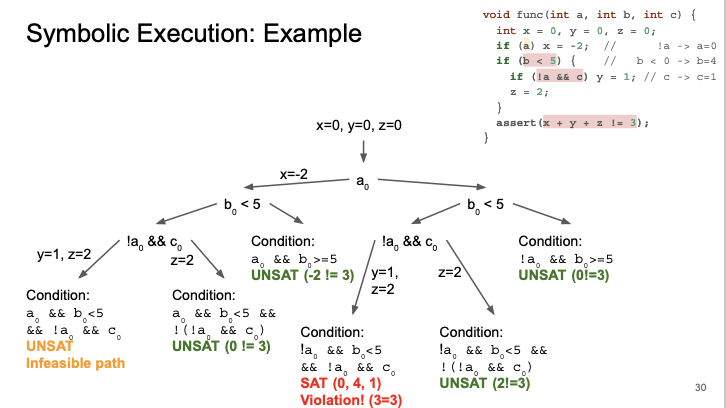
\includegraphics[width=0.8\textwidth]{symbolic-exec-example}
    \label{fig:LABEL}
\end{figure}

\section*{Concolic Execution}

Symbolic execution is limited due to state exposition (too many paths to evaluate). One way to improve is to limit the exploration close to a real path. 

\textbf{Concolic execution} starts from a real execution. abstracts it, and searches nearby. 

Path is hard-coded but remaining values are explored for violations. 

\section*{Fuzzing}

Automatic and dynamic software testing technique. 

Key concept: fastest way to test a program is to run it. 

Analogy: obstacle course
\begin{itemize}
	\item Programs are riddle with control-flow decisions
	\item Only one path can be taken at a time
	\item \verb|path[-1]| may depend on \verb|path[0:-1]|
\end{itemize}

\section*{Fuzzing Obstacles}

Fuzzers are hindered by control-flow and data-flow restrictions
\begin{itemize}
	\item \textbf{Magic byte matching}
	\item \textbf{Checksum}
	\item \textbf{Compression/Encryption}
	\item \textbf{Dependencies}
	\item \textbf{Indirection}
\end{itemize}

\section*{Fuzzer Best Practices}

A fuzzer should \textit{explore} the program
\begin{itemize}
	\item A bug cannot be found if its code is not executed
\end{itemize}

A fuzzer should \textit{trigger} bugs
\begin{itemize}
	\item Executing buggy code does not necessarily mean a bug has been triggered
\end{itemize}

A fuzzer should \textit{identify} faults
\begin{itemize}
	\item A triggered fault that goes unidentified is wasted effort
\end{itemize}

A fuzzer should be \textit{fast}
\begin{itemize}
	\item Speed is key to a fuzzer's efficiency
	\item Higher throughput = more inputs tested = higher change of triggering a bug if it exists
\end{itemize}

\section*{Types of Fuzzing}

\textbf{Blackbox Fuzzing}: Doesn't reach deep into the program. Random input generation, no feedback, no learning, move fast, break things. 

\textbf{Greybox Fuzzing}: Feedback guidance. 

Most common feedback: coverage profiles
\begin{itemize}
	\item Coverage-guided fuzzing
	\item Objective function: code coverage
	\item Metric: a execution counts of functions/lines/basic blocks/edges
\end{itemize}

Remains fast:
\begin{itemize}
	\item Instrumentation is usually lightweight
	\item Sacrifices some CPU cycles for performance benefits
\end{itemize}

\section*{Fuzzing: Input Generation}

Not all inputs are made equal. 

Mutation-based generation doesn't required specification and inputs are seen as binary blocks. Mutators transform input (bit flips, int operations). Its fast, portable, scalable. Coverage feedback an objective function for a genetic algorithm. 

Grammar-based generation does require specification for input structure and inputs are seen as parametric data. Parameters are sample, constrains are resolved to generate grammatically-valid inputs. May be slow, application-specific. It may be of interest to test exception-handling code in a program

\section*{Sanitization: Fault Detection}

Fuzzers explore the program, possibly triggering bugs in the process and unidentified bugs are useless. 

Sanitizers are fault detectors and reporters
\begin{itemize}
	\item Verify security policies at runtime
	\item Detect many violations by may be imprecise (i.e., some violations may be missed)
\end{itemize}

\section*{Sanitization}

Ideal sanitizer: detect bugs as soon as they occur. First approximation: CPU exceptions (segfault, timeouts, div by 0, int overflows)

LLVM sanitizers by policy:
\begin{itemize}
	\item \textbf{Spatial and temporal memory safety}
	\item \textbf{Language-specific behavior}
	\item \textbf{Concurrency and ownership}
\end{itemize}

LLVM sanitizers can be applied to source code, at compile time. 

Code is instrumented with checks at every possible location, e.g., just before a memory access.

Sanitization requires a model/abstraction/policy for expected behavior
\begin{itemize}
	\item How to model logic or semantic bugs? Need specification
	\item Most specification is human-readable but not machine readable
	\item Can ChatGPT help? Probably, too slow for fuzzing
\end{itemize}

\section*{Identifying Faults}

Crashes are a certain indicator of faults, but not all bugs crash. 

Sanitizers implement fault detection by enforcing security policies. 

Typical classes of bugs have existing sanitizers (e.g., memory corruption)

Real-world systems are complex and security-critical bugs can manifest as non-corrupting logic bugs, or bugs in integration

There is room for AI-guided bug detection, but it needs to be done carefully.

\section*{Comparison of Analysis}

% Quick centered image
\begin{figure}[H]
    \centering
    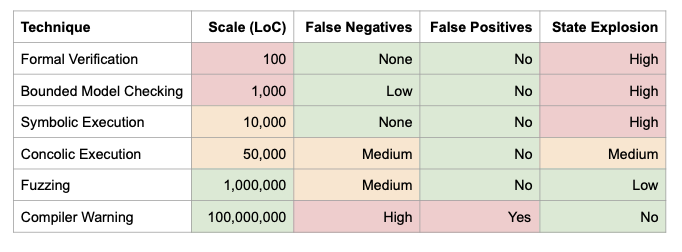
\includegraphics[width=1\textwidth]{comparison}
    \label{fig:LABEL}
\end{figure}
\end{document}
